\chapter{Mechanisms of Coronal Dimming}
\label{chaptermechanisms}

This chapter details the physics of coronal dimming. There are theoretically many physical processes that can lead to an uncareful observer identifying "dimming", which may have little to do with coronal mass ejection (CME). Traditionally, the term "coronal dimming" has been assumed to refer to the void left in the corona after a CME departs. This is one cause of a transient hole in the corona, and is of the greatest concern to space weather forecasters. Typically, a single dimming-sensitive wavelength or band will be observed and analyzed. However, changing temperatures, common during solar eruptive events, cause ionization fraction shifting, resulting in some emissions dimming while others brighten. Additionally, dark material (e.g., a filament) can pass between a bright region (e.g., flaring loops) and the observer, causing a transient dip in emission. Third, solar eruptive events sometimes have associated waves that propagate across the solar disk. These waves are observed as narrow bright fronts with a trailing dark region. The trailing dark region is another way to achieve a transient dimming of emission. Next, there are two ways that Doppler effects can cause transient dips in emission. The first is called Doppler dimming and results from fast moving plasma being sufficiently Doppler-shifted to reduce resonant fluorescence from the solar emission line sources; a phenomenon which is independent of the observation angle. The second occurs if eruptive plasma is moving fast enough in the line-of-sight to shift its emissions outside the bandpass of an observing instrument, which we have named "bandpass shift dimming". The physics, instrument effects, and mitigation strategies for each of these types of theoretically observable dimming are summarized in Table \ref{tablesummary} and are discussed in detail in the sections that follow.

\begin{table}[!h]
    \caption{Summary of physical processes that can manifest as observed dimming}
    \begin{center}
    \begin{tabular}{|p{2.5cm}|p{4cm}|p{4cm}|p{4cm}|} \hline
	Short Name & Physical Process & EVE Observational Identifiers & AIA Observational Identifiers \\ \hline \hline
	
	Mass loss \\ (Fig. \ref{massLossDimming}) & Ejection of emitting plasma from corona & Simultaneous intensity decrease in multiple coronal emission lines, with percentage decrease indicative of percentage mass lost & Area over and near the erupting active region (AR) darkens \\ \hline
	
	Thermal \\ (Fig. \ref{thermalDimming}) & Heating raises ionization states (e.g., a fraction of Fe IX becomes Fe X); cooling does the opposite & Heating: Emission loss in lines with lower peak formation temperatures and near simultaneous emission gain in lines with higher peak formation temperatures; vice versa for cooling & Heating: Area near AR darkens in channels with lower peak formation temperature and near simultaneous brightening in channels with higher peak formation temperatures; vice versa for cooling \\ \hline
	
	Obscuration (Fig. \ref{obscurationDimming}) & Dim feature (e.g., filament material) moves into line-of-sight over a bright feature (e.g., flare arcade) & Drop of emission lines proportional to their absorption cross section in the obscuring material & Direct observation of this obscuration process \\ \hline
	
	Wave \\ (Fig. \ref{waveDimming}) & Wave disturbance propagates globally, causing compression/rarefaction of plasma as wave passes by & No effects have been identified & Direct observation of this wave process, especially apparent with difference movies \\ \hline
	
	Doppler \\ (Fig. \ref{dopplerDimming}) & Fast moving plasma Doppler shifts away from resonant fluorescence with solar emission lines & Doppler wavelength shift of emission lines and change in intensity, possibly also observed as line broadening & Change in intensity of moving plasma as its velocity changes \\ \hline
	
	Bandpass \\ (Fig. \ref{bandpassDimming}) & Emissions from fast moving plasma have Doppler wavelength shift & Emission line shifts in wavelength or has broadening & Doppler shift convolves with band-pass sensitivity to cause apparent reduction in emission \\ \hline
	
	\end{tabular}
    \\ \rule{0mm}{5mm}
    \end{center}
    \label{tablesummary}
\end{table}

\section{Mass-loss Dimming}
The physical process in mass-loss dimming is the ejection of emitting plasma (see Figure \ref{massLossDimming}; \citealt{Harrison2000, Harra2001}). The ejection can be a CME or a failed ejection, the latter of which still manifests locally as a mass-loss dimming, but does not result in the appearance of a CME in coronagraph data and may not appear in a disk-integrated spectrograph like EVE. The physics model is the standard CME initiation discussed in Section \ref{sec:seePhysics}. However, where most discussions will then follow the CME as it transitions to an interplanetary CME, in mass-loss dimming we are instead interested in the details of the void left behind in the corona. The mass of an average CME and a typical active region are of the same order of magnitude: $10^{15}\ g$, meaning that a departing CME can "blow out" a large part of the active region with it \citep{Aschwanden2009}. This is the physical process assumed to be the main contributor to observed dimming in many recent studies \citep{Sterling1997, Reinard2008, Reinard2009, Aschwanden2009}. \citet{Harrison2003} showed that dimmings can account for a large percentage of CME mass. Thus, mass-loss dimming is very relevant for the space weather community.

\begin{figure}[!b]
	\caption[Schematic of mass-loss dimming]{
	    Schematic depicting the process of mass-loss dimming. Prior to the eruption (left), coronal loops are relatively 
	    quiescent. During and after the eruption (right), the loops are brighter and reconfigured, a CME is ejected, and a 
	    void forms in the coronal plasma.
	}
    \begin{center}
	    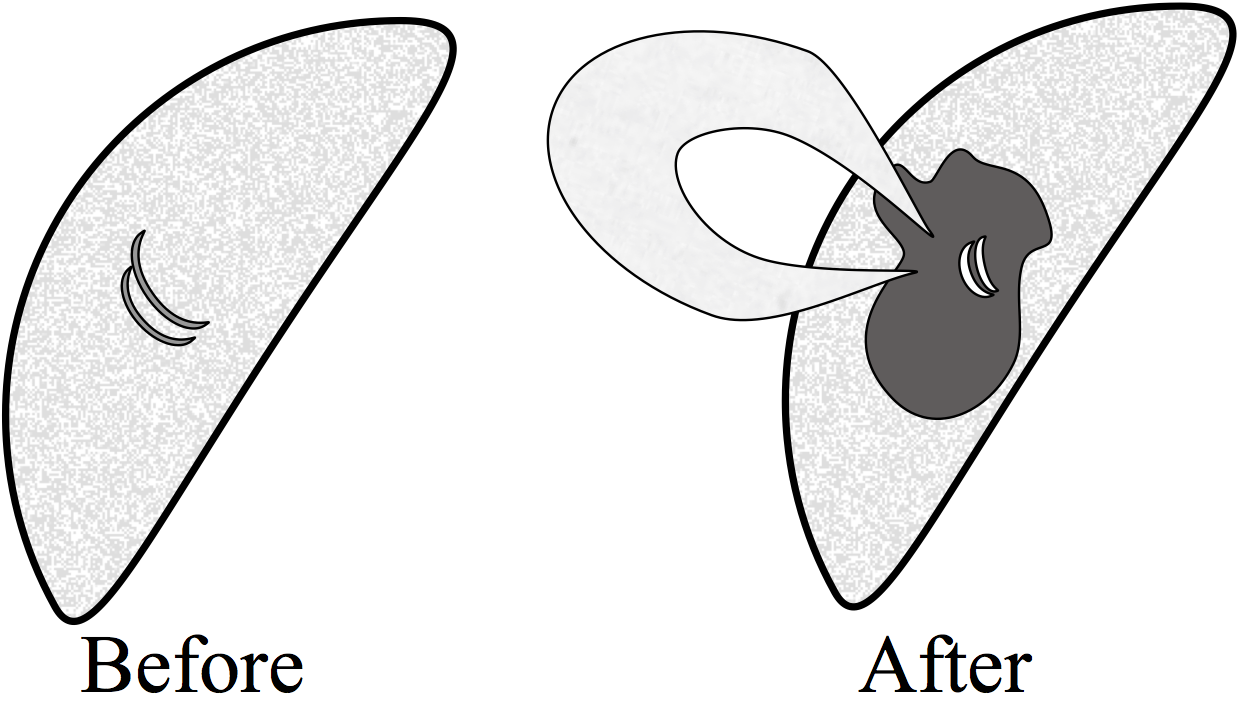
\includegraphics[width=100mm]{Images/MassLossDimming.png}
    \end{center}
    \label{massLossDimming}
\end{figure}

Observationally, mass-loss dimming appears in EVE as multiple emission lines dropping nearly simultaneously. In the case of a failed ejection, the dimming area and the ejected material are likely to maintain a total emission that is close enough to constant that it will not be apparent in EVE data. For space weather, this is of little concern since CMEs have far greater geoeffectiveness than short-lived holes in the corona of small spatial extent. However, AIA data allow the identification of mass-loss dimming even if the event is a failed ejection. In either case, mass-loss dimming appears in AIA as a relatively compact area near an active region becoming darker, sometimes with a dark cloud visibly moving off-disk. Assuming the dimmings in \citet{Reinard2008} to all be due to mass loss, the timescale of the process is 3–12 hr and rarely persists longer than a day. Additional observations from the Hinode spacecraft have confirmed density decreases with accompanying outflows \citep{Attrill2010, Harra2010, Tian2012}.

\section{Thermal Dimming}
Temperature evolution of emission lines is only interpreted as observed dimming if one is not careful to observe co-spatial emission lines at different peak formation temperatures. As plasma is heated or cooled, the ionization fraction changes, necessarily causing the emission intensity to change (Figure \ref{thermalDimming}). For example, heating causes some Fe IX to become Fe X and thus, in the absence of competing physical processes, 171 \AA\ emission drops while 177 \AA\ rises. This pattern was identified observationally in Figure 6 of \citet{Woods2011} using SDO/EVE data, \citet{Robbrecht2010} using STEREO/EUVI, \citet{Jin2009} and \citet{Imada2007} with Hinode/EIS. It can also be observed in the standard composite (multi-wavelength) movies produced by the AIA team; indeed, this is one of the prime purposes for the composites. The initiation time and duration of temperature evolution tends to be quite similar to mass-loss dimming, as they are typically both responses to the rapid release of magnetic field energy in active regions and require several hours of recovery time. Thus, thermal processes could be mistaken for mass loss if only a single spectral line was observed. Ideally, unblended emission lines from an entire coronal ionization sequence (e.g., Fe I to Fe XVIII) could be used to mitigate this convolution of dimming observations. However, as we will show in Section 4.3, it may be sufficient to have observations of two sufficiently separated ionizations states to differentiate between thermal evolution and mass-loss dimming. This is due, in part, to the fact that hotter lines (e.g., Fe XV and above) are primarily emitted from confined loops near the flare and are thus not strongly impacted by mass-loss dimming. Multi-wavelength Doppler studies have shown that while all (measured) emission lines become blue-shifted (indicating an outflow), the magnitude of the shift is strongly directly proportional to the lines peak formation temperature \citep{Imada2007, Jin2009}. Figure \ref{upflowVsTemperature} shows this dependence for a plage region with a dimming during an X-class flare. In particular, Fe IX 171 \AA\ emission can be depressed further after open magnetic field lines from the departing CME close down and cause another bout of heating; causing e.g., Fe IX to become Fe X and beyond, which propagates outward as a "heat wave dimming" \citep{Robbrecht2010}. It may even be that cool emissions like Fe IX 171 \AA\ are simply moving too slow to account for mass depletion and that warmer lines, such as Fe XII 195 \AA\ better represent the mass being ejected \citep{Robbrecht2010}. However, \citet{Mason2014} found that the onset time, slope, and duration of dimming are comparable in SDO/AIA 171 \AA\ and 193 \AA\footnote{Note that the SDO/AIA 193 \AA\ band encompasses 195 \AA\ }and in SDO/EVE 171 \AA\ and 195 \AA\ (described in Chapter \ref{chaptercasestudy}). 

\begin{figure}[!htb]
	\caption[Schematic of thermal dimming]{
	    Schematic depicting the observational difference between dimming and non-dimming emission
	    lines. Relative to a pre-eruption time (left), the Fe IX emission drops while the Fe XIV
	    emission increases (right) due to heating of the plasma and redistribution of ionization
	    states.
	}
    \begin{center}
	    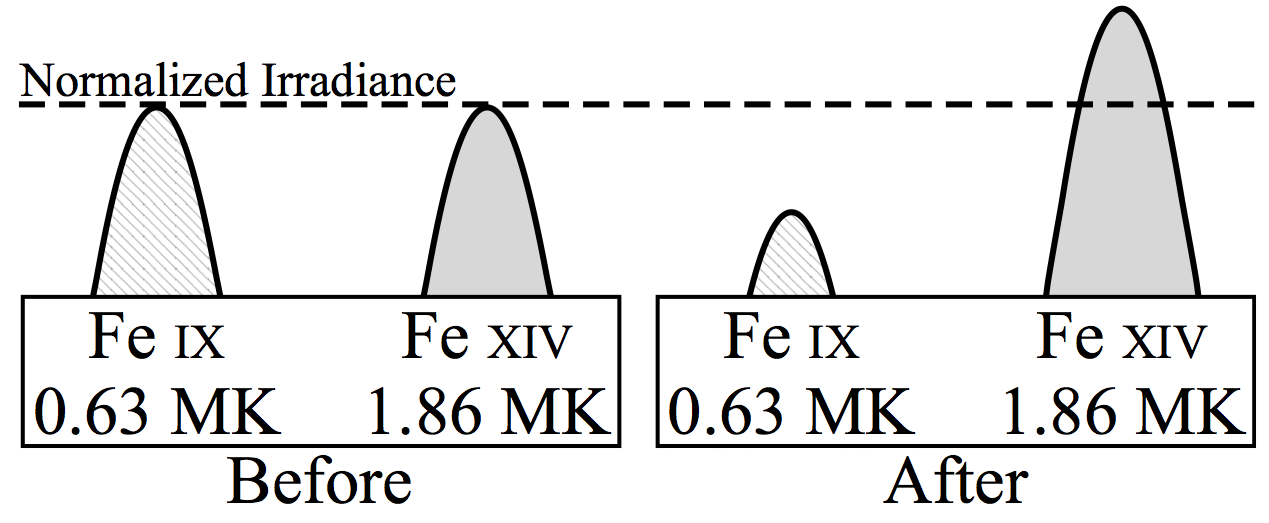
\includegraphics[width=100mm]{Images/ThermalDimming.png}
    \end{center}
    \label{thermalDimming}
\end{figure}

\begin{figure}[!htb]
    \caption[Outflow velocity vs temperature]{
        Outflow velocity vs emission line peak formation temperature for a dimming region near a plage. 
        Adapted from \citet{Imada2007}.
        }
    \begin{center}
        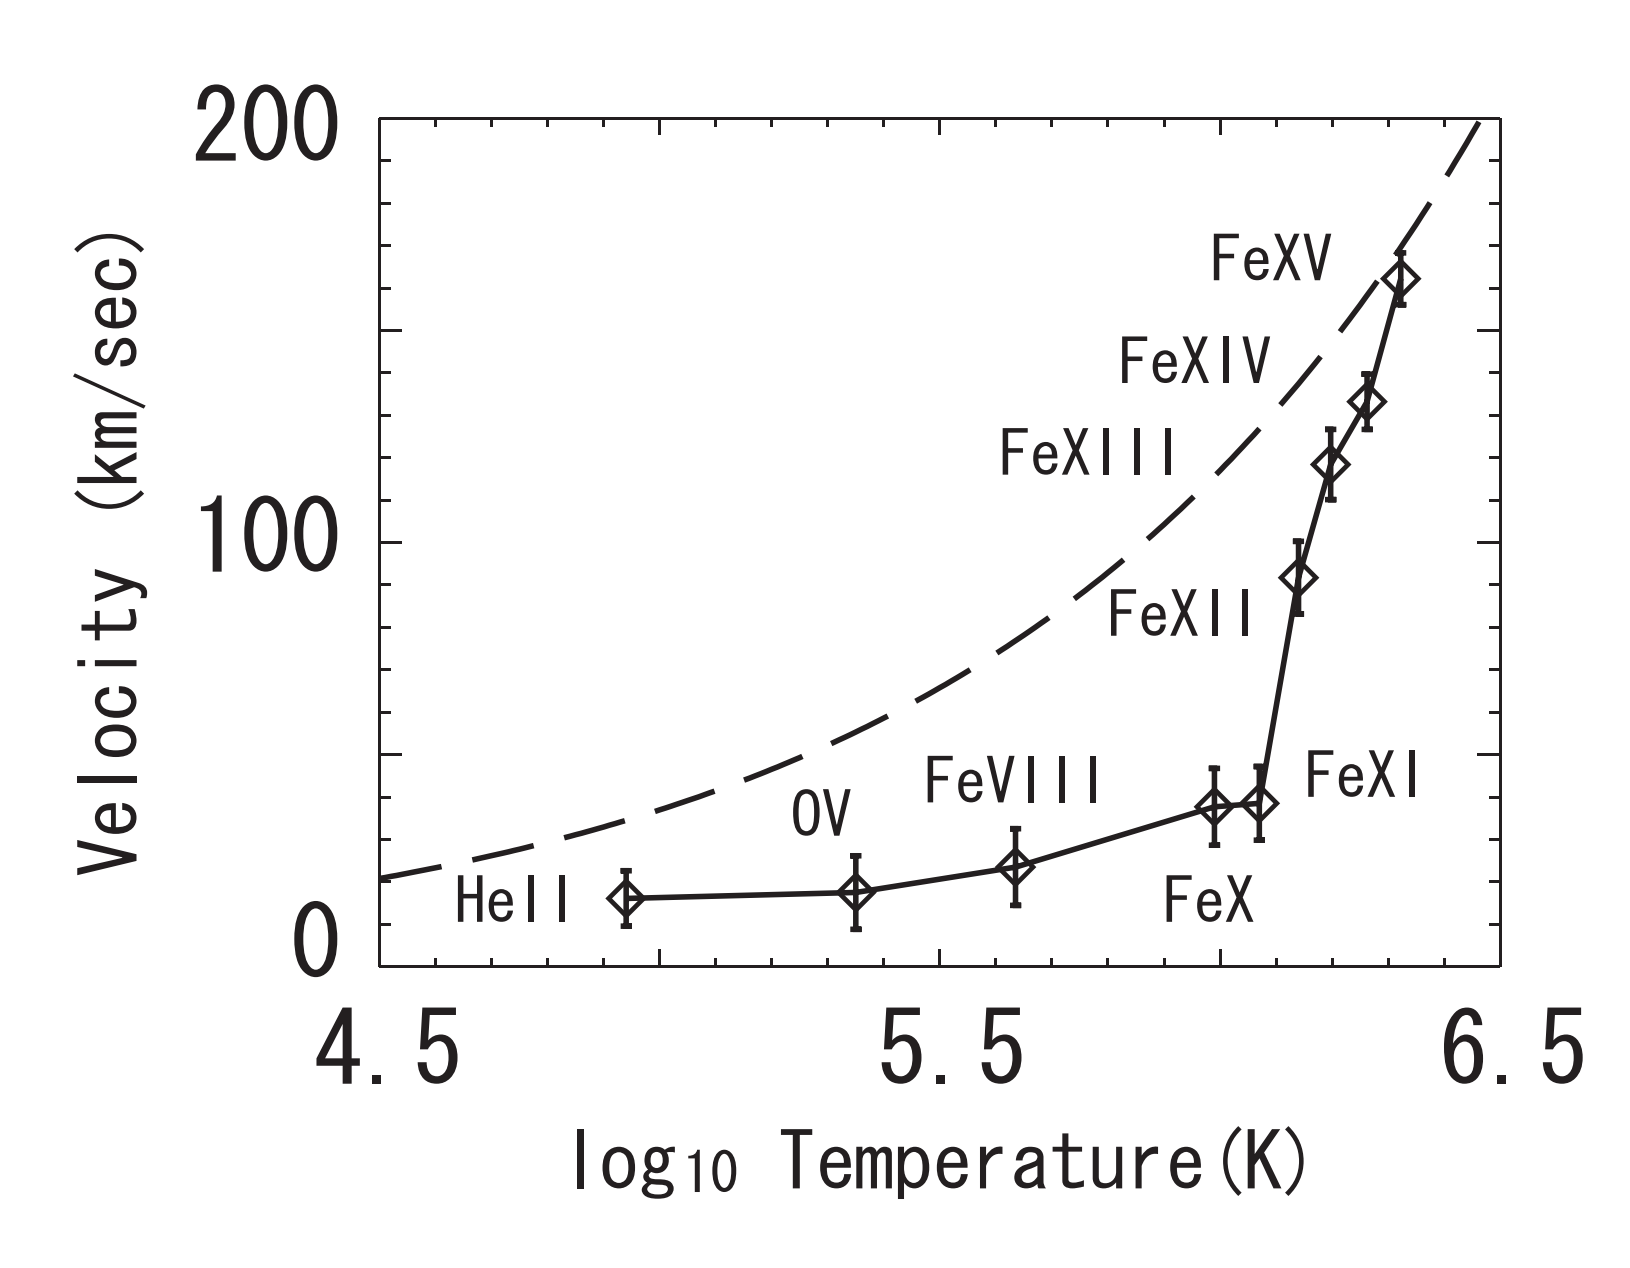
\includegraphics[width=90mm]{Images/UpflowVsTemperature.png}
    \end{center}
    \label{upflowVsTemperature}    
\end{figure}


It is important to note that, in general, the magnitude of total observed dimming in a given line in EVE spectra is inversely proportional to its peak formation temperature, which can be inferred from Figure \ref{detectedDimmingVsIonization}. This figure was generated using a simple algorithm that searched all EVE/MEGS-A data for relative irradiance decreases greater than a specified threshold (1\%, 2\%, 3\%) of flares exceeding GOES X-ray class of C1. The window of time searched was bounded by the GOES event start time and the sooner of either 4 hours after the start time or the next GOES event start time. This algorithm was applied to all EVE data from mission start (2010 February 10) to the failure of the MEGS-A instrument (2014 May 26). MEGS-A takes the measurements of all wavelengths studied here. Figure \ref{detectedDimmingVsIonization} shows that the number of dimmings dramatically decreases as the magnitude threshold is increased, and decreases slightly with higher peak formation temperature. This latter effect is partially due to flare heating adding emission in the higher temperature, higher ionization state, lines that partially offsets the mass-loss dimming. Additionally, these trends indicate that at sufficiently high peak formation temperature, no dimming may be observed at all, even at the lowest detection threshold, which is consistent with the hotter lines being restricted to the confined flare loops and hence experiencing no mass loss. In other words, the higher the peak formation temperature, the greater the relative contribution of more confined loops to the measured emission. 

\begin{figure}[!h]
    \caption[Dimming dependence on temperature in EVE]{
        Number of identified dimmings in EVE for six spectral lines using different percentage dimming depths as the
        threshold for a detection. There were 263 flares used to trigger an automated search for dimming in EVE. 
        Note the decrease in detections with increasing ionization state (i.e. peak formation temperature).
    }
    \begin{center}
        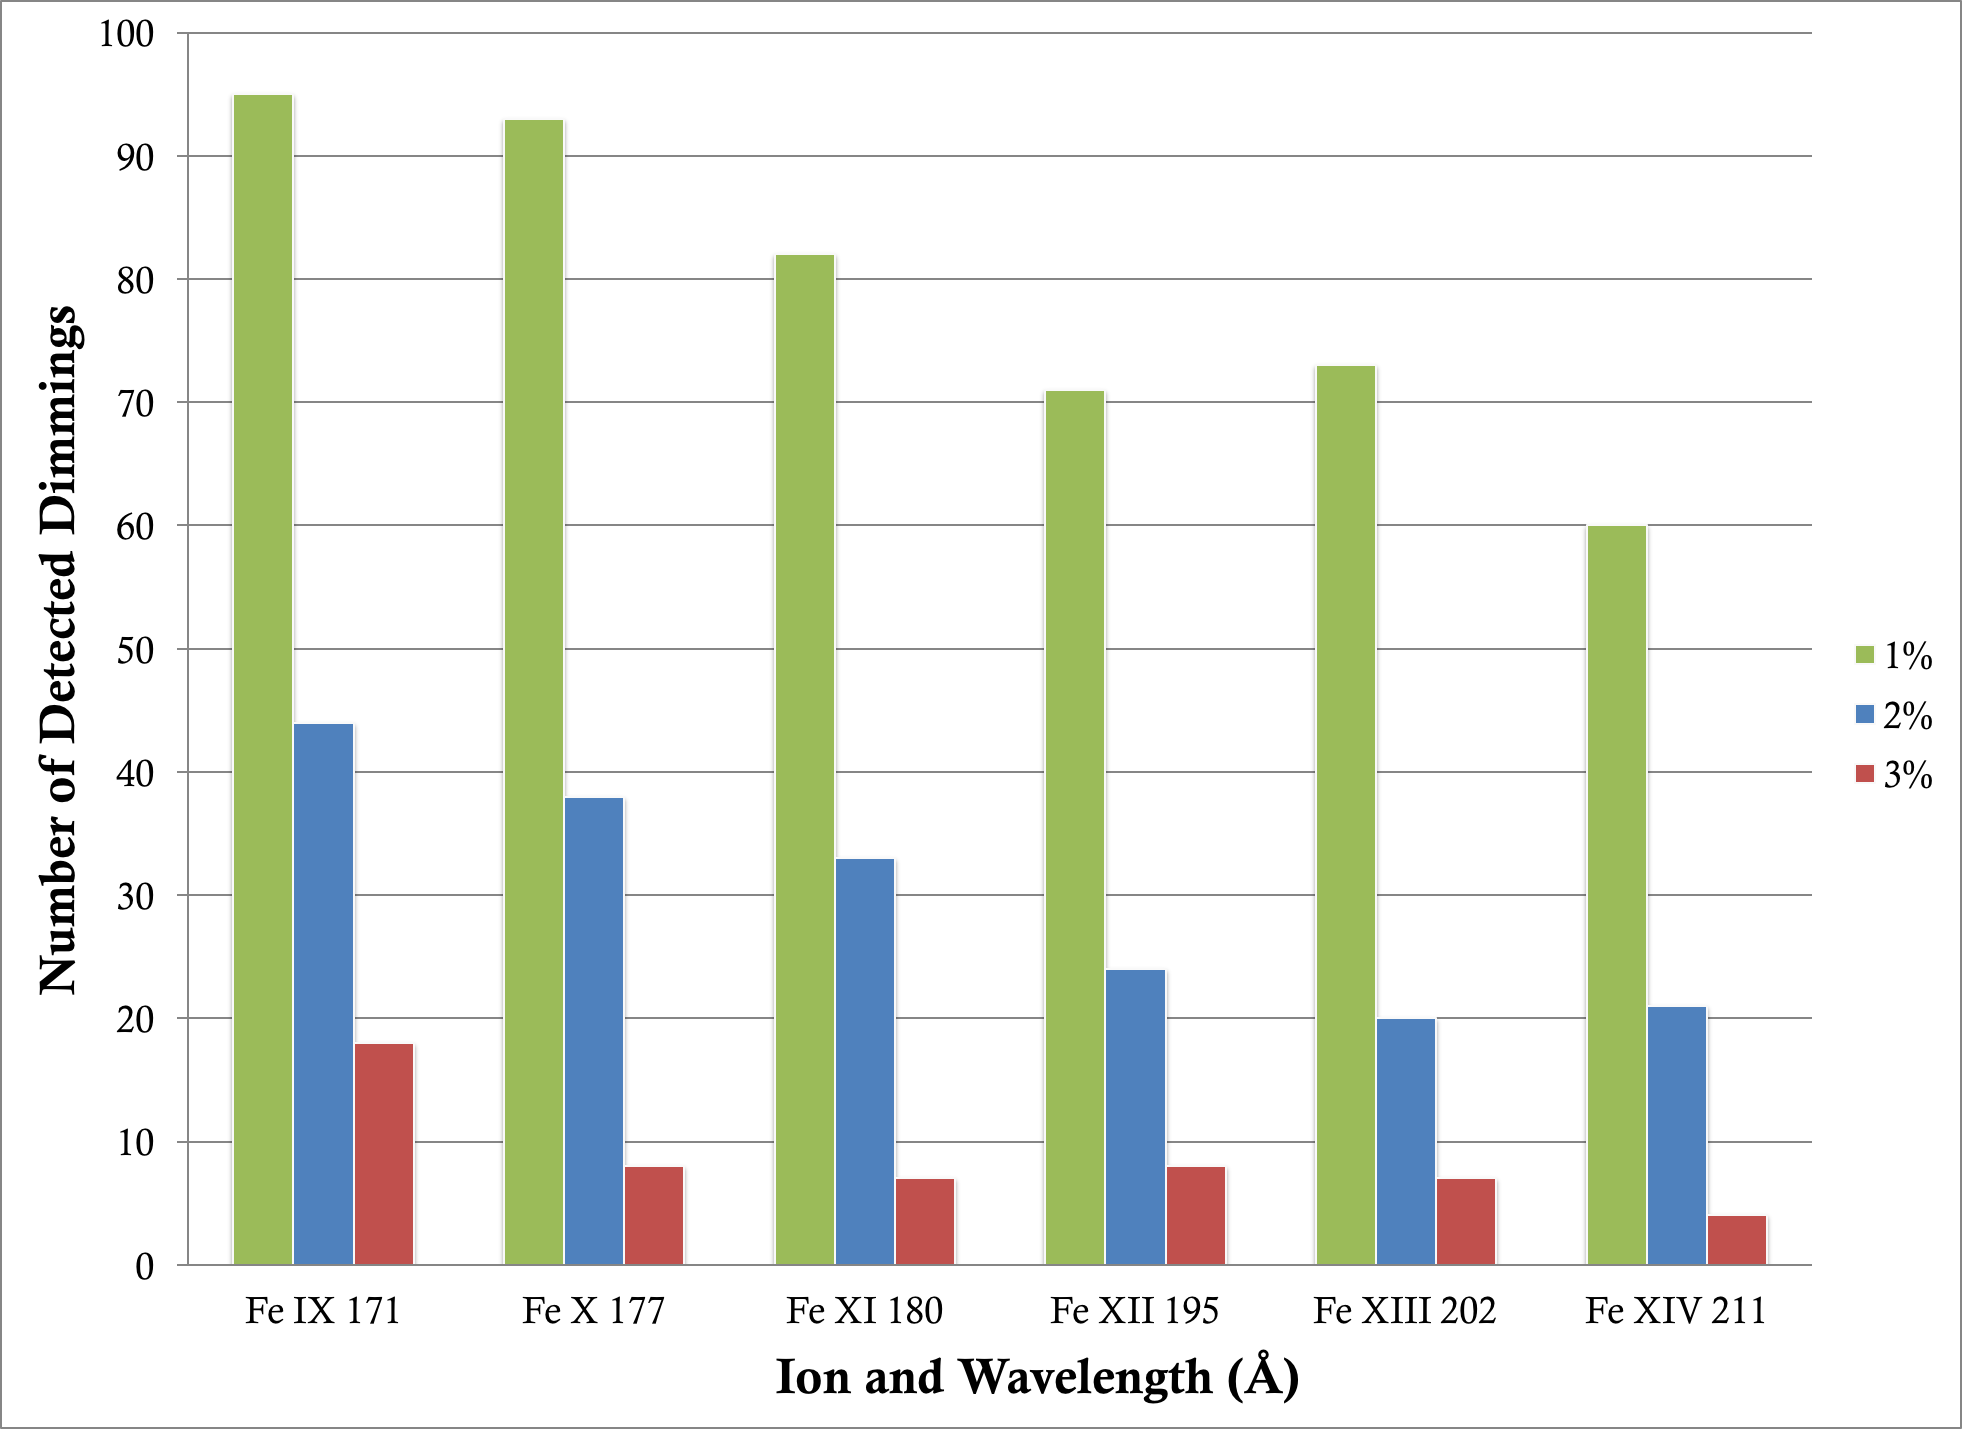
\includegraphics[width=150mm]{Images/DetectedDimmingVsIonization.png}
    \end{center}
    \label{detectedDimmingVsIonization}
\end{figure}

An instrument with spatial resolution like AIA can be used to isolate the confined flaring loops and create a time series of just the dimming region, and this is a procedure carried out in Chapter \ref{chaptercasestudy}. AIA too has its own limitations: relevant in this case is the relatively lower spectral resolution that blends together emission from several ionization states of Fe. With EVE and AIA combined, it is possible to analyze thermal dimming but the idea instrument for fully characterizing this phenomenon would be a high-resolution hyperspectral imager in the EUV.

\section{Obscuration Dimming}
The physical process that results in apparent dimming here is material that is dark in a particular wavelength (e.g., a filament) moving between bright material (e.g., flare arcade) and the observer (Figure \ref{obscurationDimming}). In optically thick wavelengths, the dark plasma absorbs some of the bright emission, resulting in an apparent decrease in emission. The slow draining of plasma back to the corona can obscure underlying emission for hours, and absorption can be observed in both coronal and chromospheric lines (e.g., \citet{Gilbert2013}). Although the obscuration dimmings can exhibit time and spatial scales comparable to the more short-lived mass-loss dimmings, it is fairly straightforward to identify absorption signatures in the EUV images. It may also be possible to identify this phenomenon with EVE using the He II 256 \AA\ and 304 \AA\ chromospheric emission lines and knowledge of the absorption cross-section through filamentary plasma. Figure \ref{photoionizationCrossSection} shows the photoionization cross-sections of the dominant species in the solar corona. Hydrogen and helium contribute an order-of-magnitude more absorption than metals\footnote{"Metals" in the astrophysical sense}, and thus the effect of metals can be ignored. The cross-sections are quite steep in the wavelength range of interest here (roughly 150-310 \AA). This means that approximately twice as much He II 256 \AA\ than He II 304 \AA\ emission will come through a filament. Furthermore, the mass-loss dimming sensitive lines (e.g., Fe IX 171 \AA\ and 195 \AA) will be less affected by this obscuration, but a 1\% effect would be sufficient to cause a "false" detection. It may be possible to identify obscuration dimming with EVE's 256 \AA\ and 304 \AA\ measurements and determine that an obscuration dimming has occurred. However, further analysis of this type of dimming is required before any conclusions can be drawn. 

\begin{figure}[!h]
    \caption[Schematic of obscuration dimming]{
        Schematic depicting the process of obscuration dimming. A filament previously obscuring only the quiet Sun (left)
        expands and moves in front of a flare arcade (right). This results in a decreased observed emission from the flare
        arcade in wavelengths where the filament is optically thick.
    }
    \begin{center}
        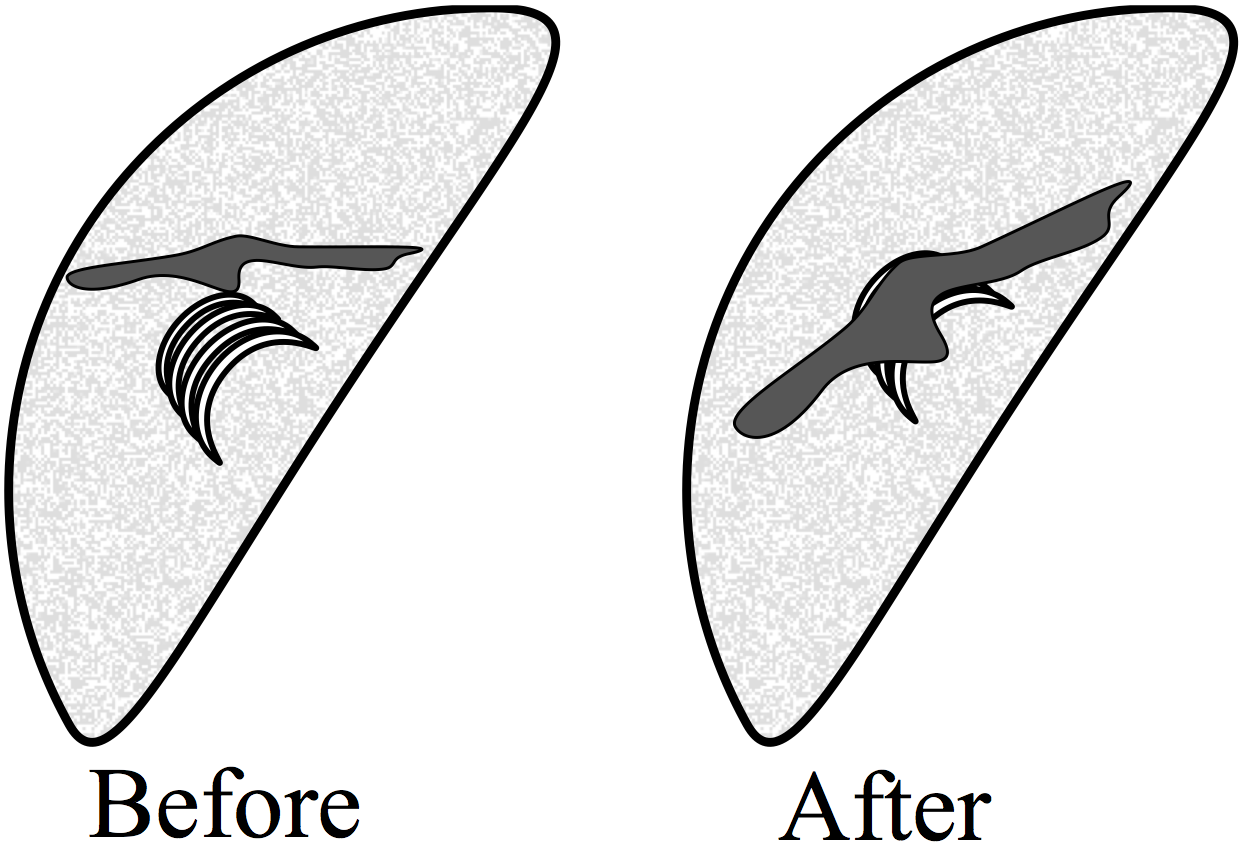
\includegraphics[width=75mm]{Images/ObscurationDimming.png}
    \end{center}
    \label{obscurationDimming}
\end{figure}

\begin{figure}[!h]
    \caption[Photoionization cross-sections for H and He]{
        Photoionization cross-sections for He I (dot-dashed line), He II (solid line), and H (dashed line) per hydrogen
        atom. The inset shows a wider wavelength range of the same data but with metals shown for comparison. The dashed
        vertical bars at the bottom indicate the edges of respective continua. The grey regions at the bottom are not 
        pertinent here as they correspond to specifics of the SOHO/CDS instrument. Adapted from \citet{Andretta2003}. 
    }
    \begin{center}
        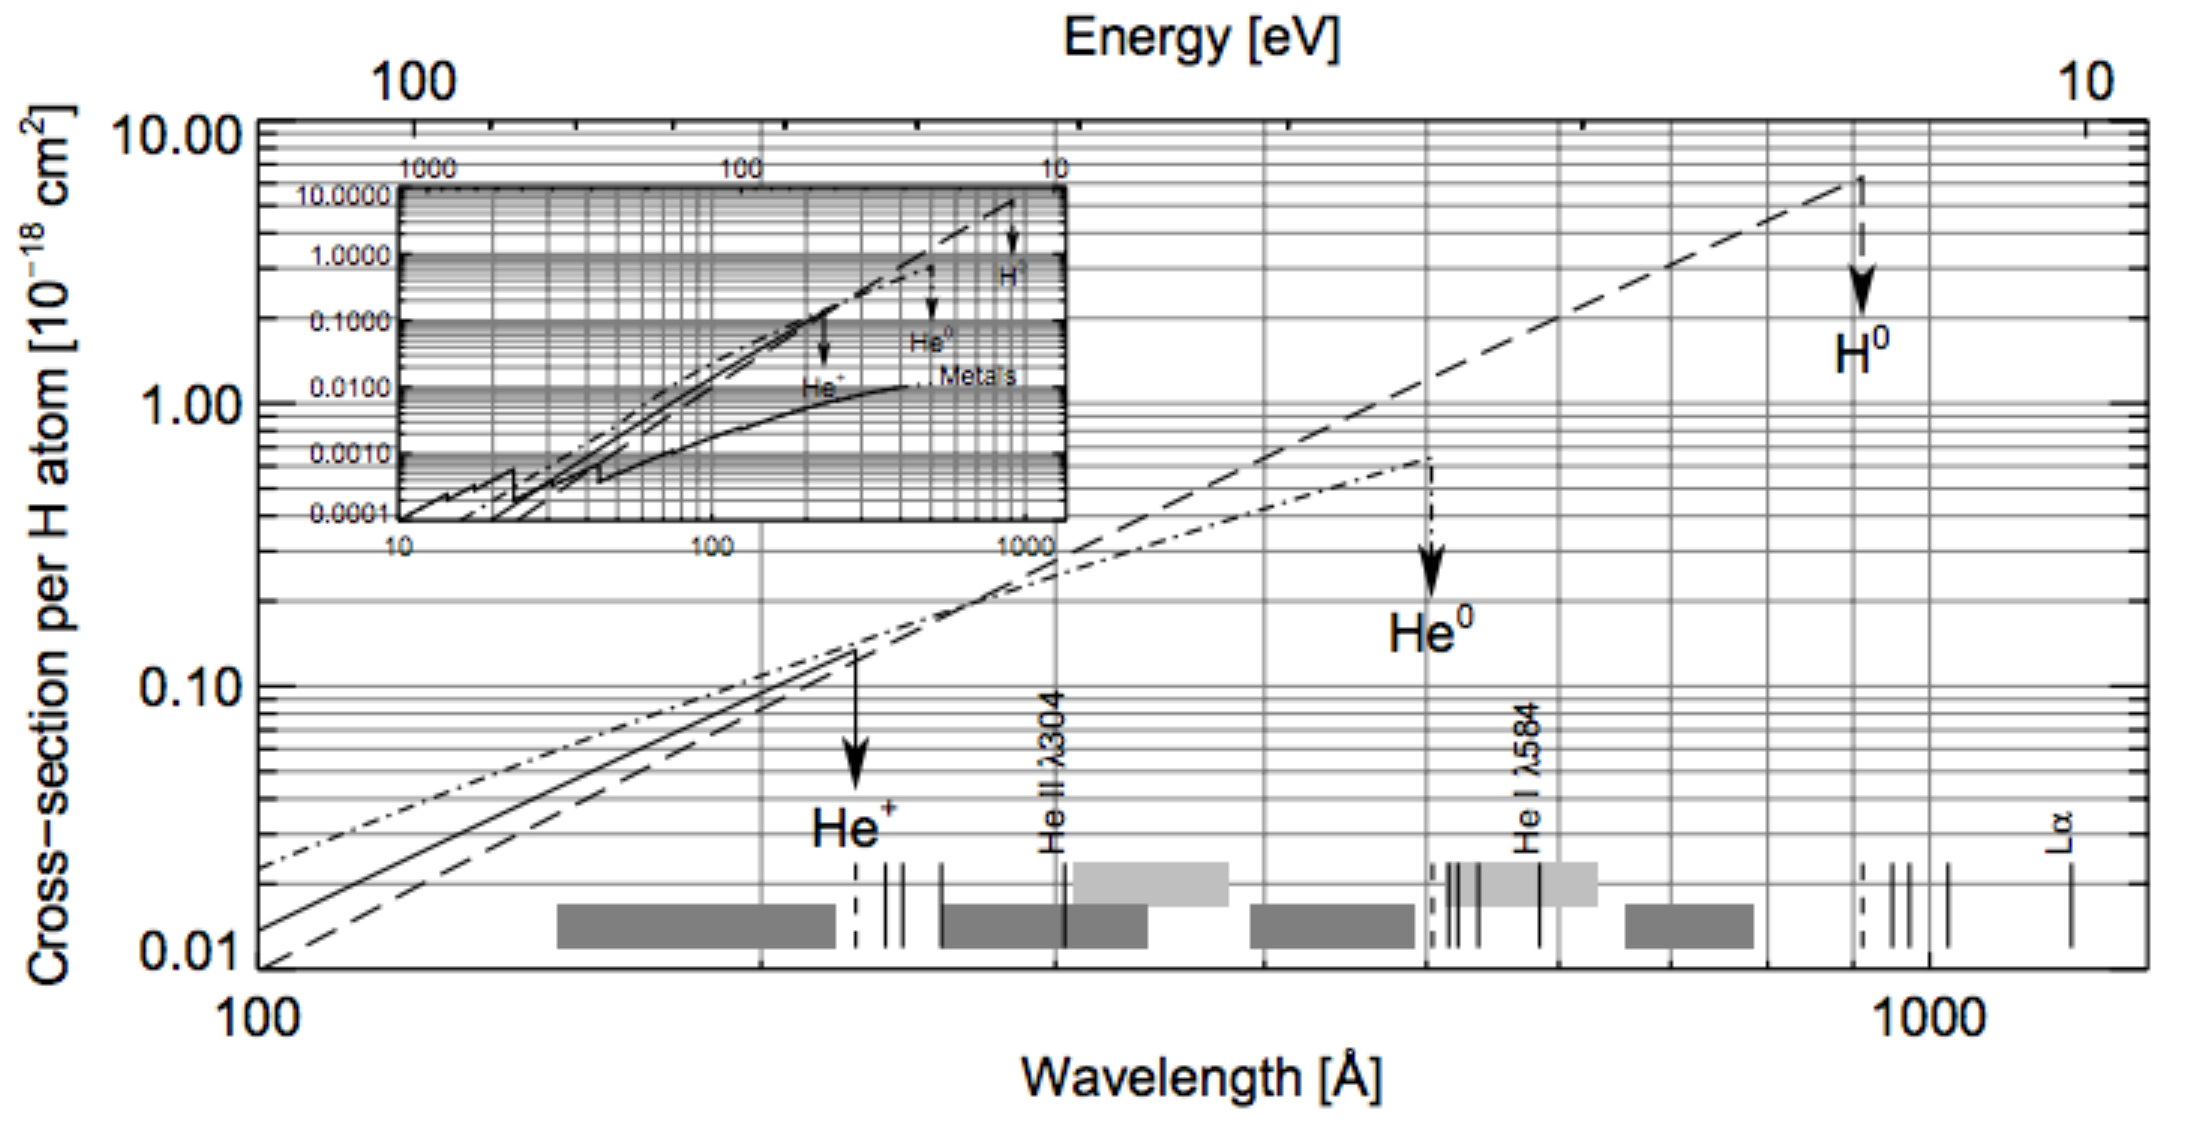
\includegraphics[width=150mm]{Images/PhotoionizationCrossSection.png}
    \end{center}
    \label{photoionizationCrossSection}
\end{figure}

\section{Wave Dimming}
\label{sec:waveDimming}
The debate about the physics of coronal “EUV waves” continues (e.g., \citet{Zhukov2004, Muhr2011, Liu2014}) but one of the simplest explanations of the observations is that plasma is compressed as a longitudinal wave passes through the medium. Traveling (i.e., not static) rarefactions are sometimes observed following the compression \citep{Muhr2011}, the compressed regions having higher densities resulting in increased emission, and vice versa (Figure \ref{waveDimming}). Alternatively, some models suggest that the observed phenomenon is not a wave at all, but rather the impact of the CME departing on the global magnetic field \citep{Chen2002, Chen2005}. Regardless of the physical process responsible, the observation is the same. The EUV waves emanating from an eruption can be seen to cause dimmings and brightenings elsewhere in the solar EUV images, often very far from the original eruption site, particularly near other active regions. We refer to these dimmings that are non-local to the erupting site as “sympathetic dimmings.”

\begin{figure}[!h]
    \caption[Schematic of obscuration dimming]{
        Similar to Figure \ref{obscurationDimming}, but depicting the process of wave dimming. After an eruptive event, a 
        wave propagates and expands through the corona. The compressed plasma of the wavefront results in enhanced emission,
        while the rarefied trailing region is dimmed. 
    }
    \begin{center}
        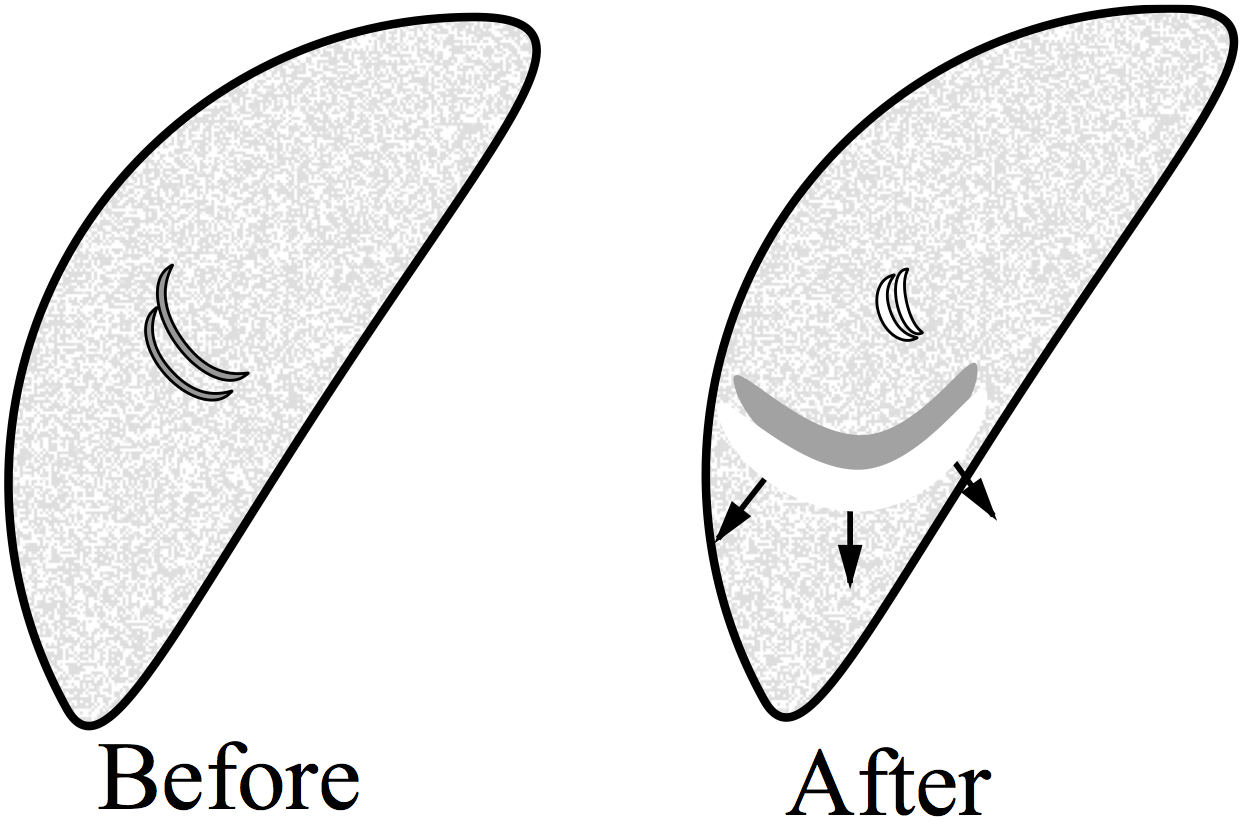
\includegraphics[width=75mm]{Images/WaveDimming.png}
    \end{center}
    \label{waveDimming}
\end{figure}

It is important to distinguish between the wave-caused dimmings and other causes of remote dimming, such as large-scale disappearing loops that are visible in soft X-ray images but only have visible EUV changes at their footpoints \citep{Pohjolainen2005}. EUV wave dimmings are unlikely to be easily identified in full-disk spatially-integrated instruments like EVE because the enhanced emission nearly cancels out the dimmed emission when summed. However, the global nature of these events has the potential to trigger eruptive events in distant regions \citep{Schrijver2015}, potentially leading to further dimming. This is quite likely to occur if a distant active region has significant potential energy stored when the disturbance reaches it -- the wave propagating across the magnetic field lines acts as a catalyst. 

\section{Doppler and Bandpass Dimming}
Two additional processes can theoretically lead to the observation of dimming in a limited wavelength range; both result from Doppler effects. The first has been given the name "Doppler dimming". In this type of dimming, resonant fluorescence of a high-velocity, remote cloud of plasma (e.g., CME) by a source population (solar emission lines) can decrease as the resultant Doppler shift becomes sufficiently large (see Figure \ref{dopplerDimming}; \citealt{Hyder1970}). Here, Doppler takes effect due to the relative velocity between the source (the Sun) and the scattering medium (the CME) and is thus independent of observer angle. This phenomenon has been known for decades for cometary emissions \citep{Swings1941, Greenstein1958} and has been documented in chromospheric lines associated with eruptions \citep{Labrosse2012} as well as in coronal lines such as O VI for polar coronal hole outflows \citep{Giordano2000}. However, the majority of EUV emission lines in the corona are collisionally dominated i.e. not resonantly excited, and will not exhibit this effect. Furthermore, the dimming region is the CME itself, which is likely to be outside the field of view of EUV instruments observing the solar disk. Therefore, it is possible to diagnose this type of dimming when it is pronounced in resonantly excited lines but does not manifest in the lines of interest studied herein. 

\begin{figure}[!h]
    \caption[Geometry and effect of Doppler dimming]{
        (a) Geometry of Doppler dimming. The large circle at the bottom represents the Sun, the point P represents the 
        position of mass that has erupted e.g., a CME. The vector V is the velocity of the CME. The square patch on the Sun
        represents an area of source emission. Adapted from \citet{Rompolt1967a}. (b) The H$\alpha$ profiles seen by (A)  a 
        stationary observer at a height of 5600 $km$ above the photosphere; and (B) an observer at a height of 30,000 $km$ 
        moving radially outward at 75 $km\ s^{-1}$. The mean intensity (as seen by the scattering medium) is measured in 
        units of the intensity of the nearby continuum at the center of the disk. It can be seen that the Doppler shift 
        also causes an intensity decrease. Adapted from \citet{Hyder1970}. 
    }
    \begin{center}
        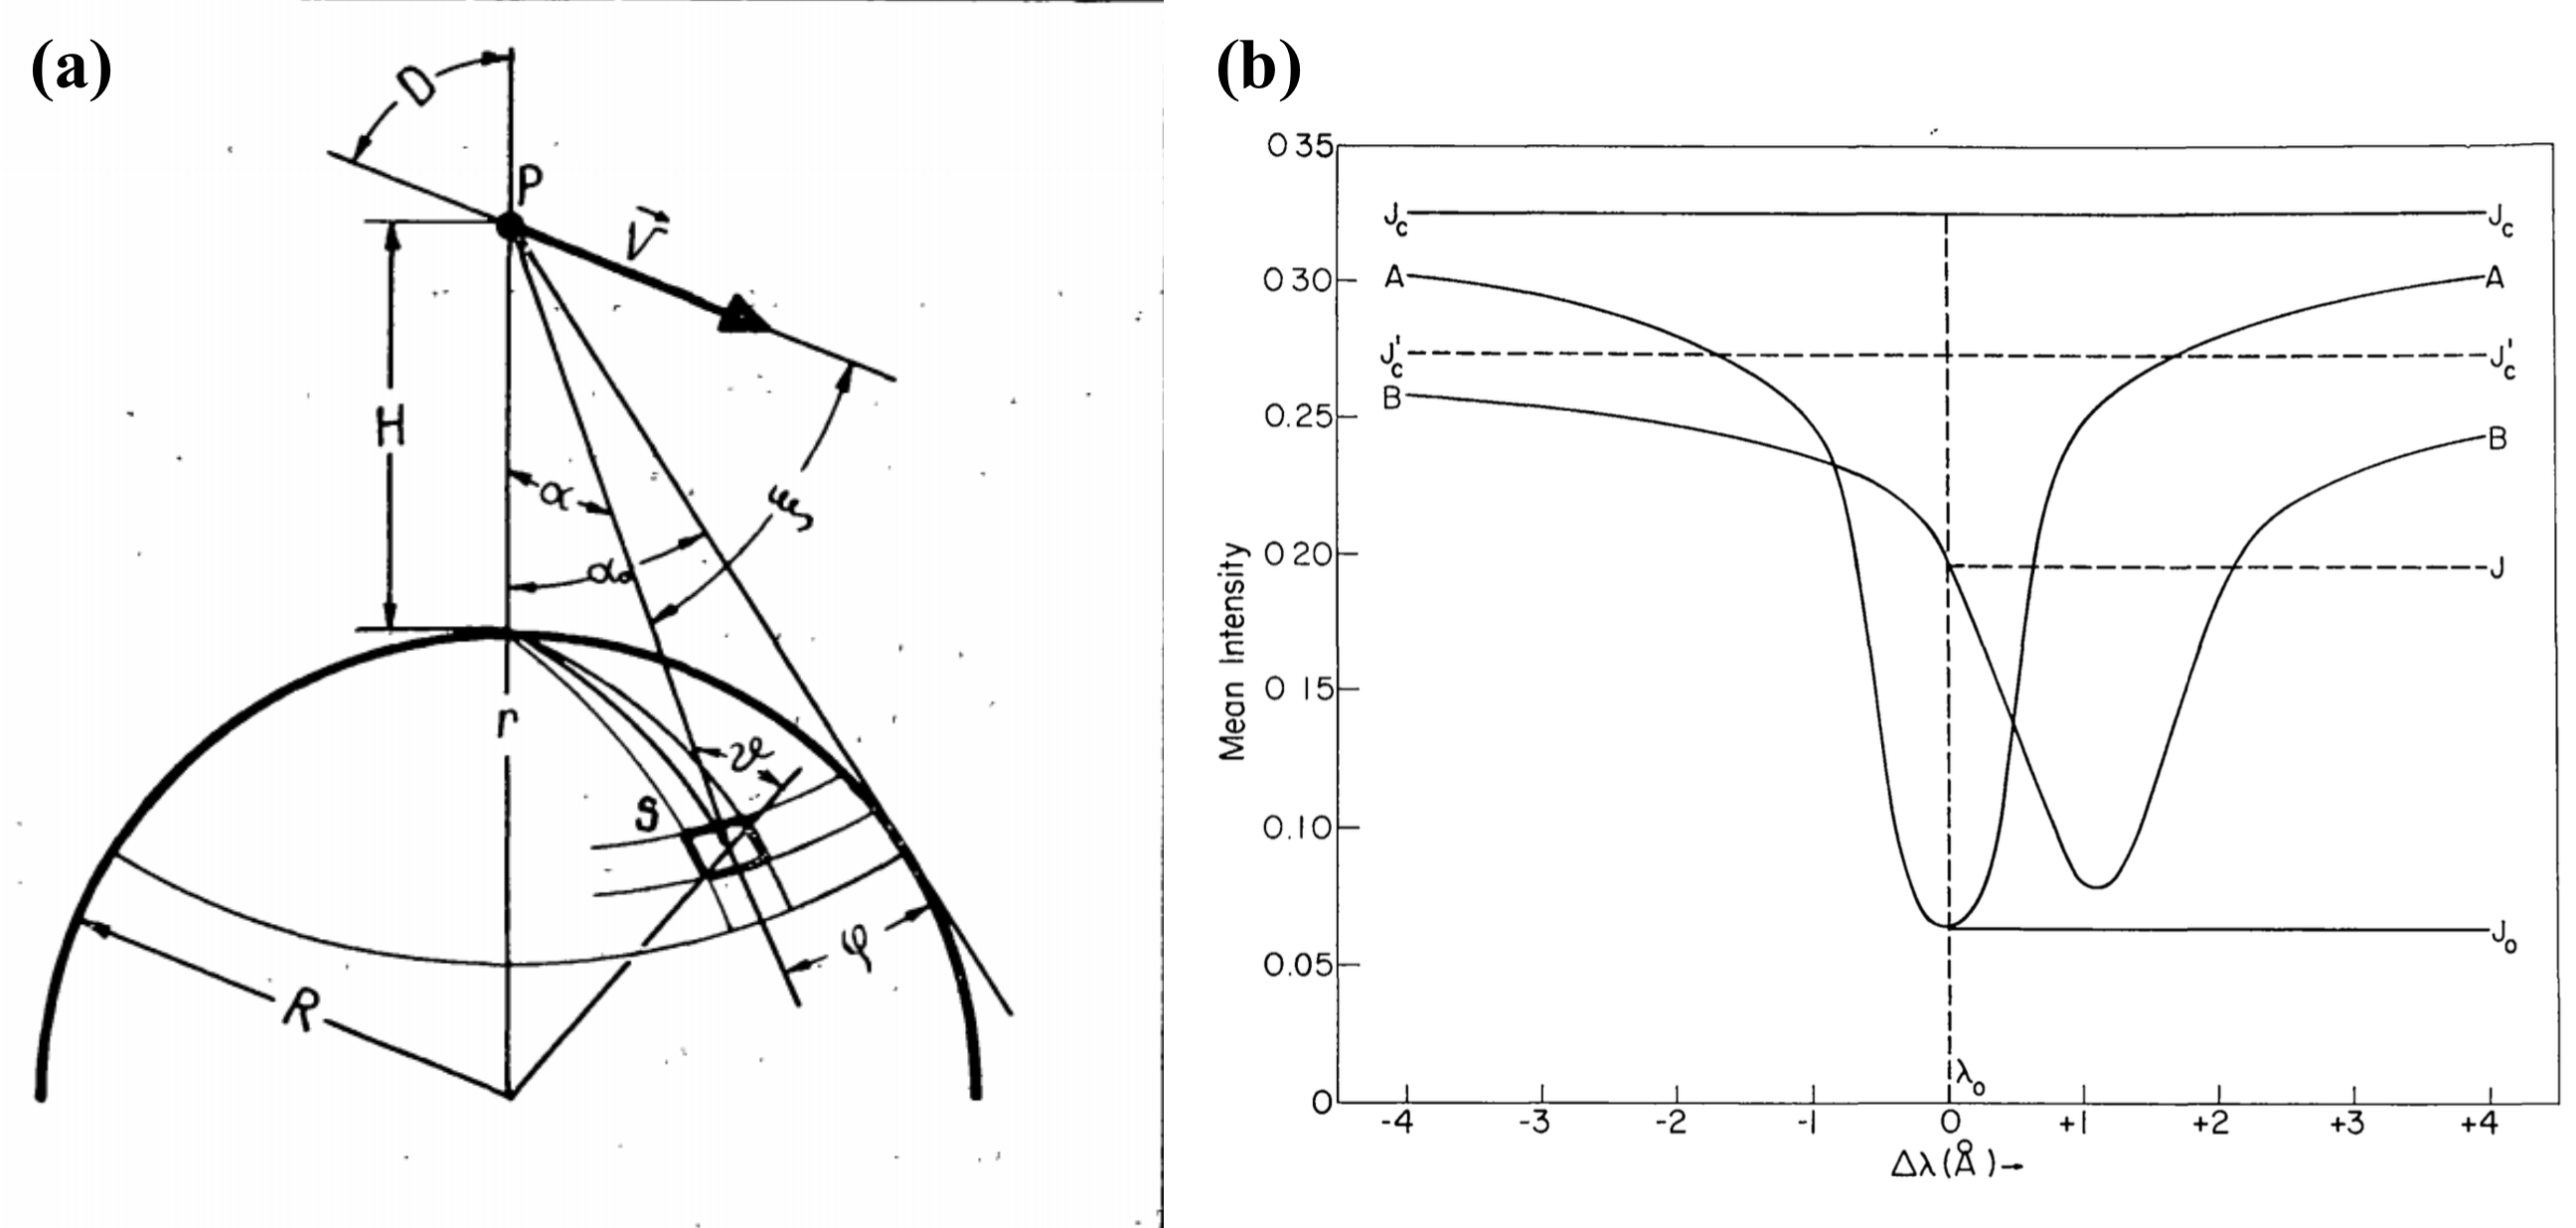
\includegraphics[width=150mm]{Images/DopplerDimming.png}
    \end{center}
    \label{dopplerDimming}
\end{figure}

The second type of dimming that results from a Doppler effect is one we call "bandpass dimming". This physical process is tied to the observer’s location similarly to obscuration dimming (see Section \ref{obscurationDimming}). Mass ejected toward the observer will have emissions that are necessarily blue-shifted. If the velocity was high enough, it could shift emission lines outside of an imager's bandpass, causing an apparent dimming in the data. Most imagers use filters that tend to have bandpasses on the order of nanometers but can have sharp edges (Figure \ref{bandpassDimming}). CMEs typically have speeds ranging from a few hundred to a couple thousand $km\ s^{-1}$. However, a CME only accounts for a small fraction of the total emission from the solar disk. As noted in \citet{Hudson2011}, these Doppler shifts tend to be on the order of picometers. Additionally, a CME moving fast enough to shift emission outside the bandpass would be outside the field-of-view of the instrument in a very short time. Thus, this type of apparent dimming is not expected in EUV images, but we include it for completeness and note that this may be a consideration for future instrumentation. 

In a spectrograph like EVE, the Doppler shifts would instead simply cause a wavelength shift of the emission line from the ejected material, which is how \citet{Hudson2011} performed their analysis. When this Doppler-shifted emission is convolved with the relatively static plasma remaining on the Sun, a small Doppler shift from the ejected material manifests as line-broadening in the integrated irradiance while a large shift would result in a line splitting. It should be noted that the EVE extracted lines data product applies a static mask to the spectra so a sufficiently large Doppler shift could cause an apparent dimming in this product. Again, the observed shifts are far too small to impact the EVE data analysis.

\begin{figure}[!h]
    \caption[Bandpass dimming]{
        (a) and (b) are snapshots from a movie produced by Barbara Thompson. 
        (a) Bottom: The dashed line shows a modeled solar spectrum and the solid line shows the bandpass for AIA's 171 \AA. 
        Top left: The ratio of emission relative to plasma with no line-of-sight velocity as a function of velocity. 
        Top right: The amount of density decrease (in \%) that would be required to achieve the same amount of dimming as 
        bandpass dimming at each velocity. 
        (b) Same as (a) but at a velocity of 1053 $km\ s^{-1}$. 
    }
    \begin{center}
        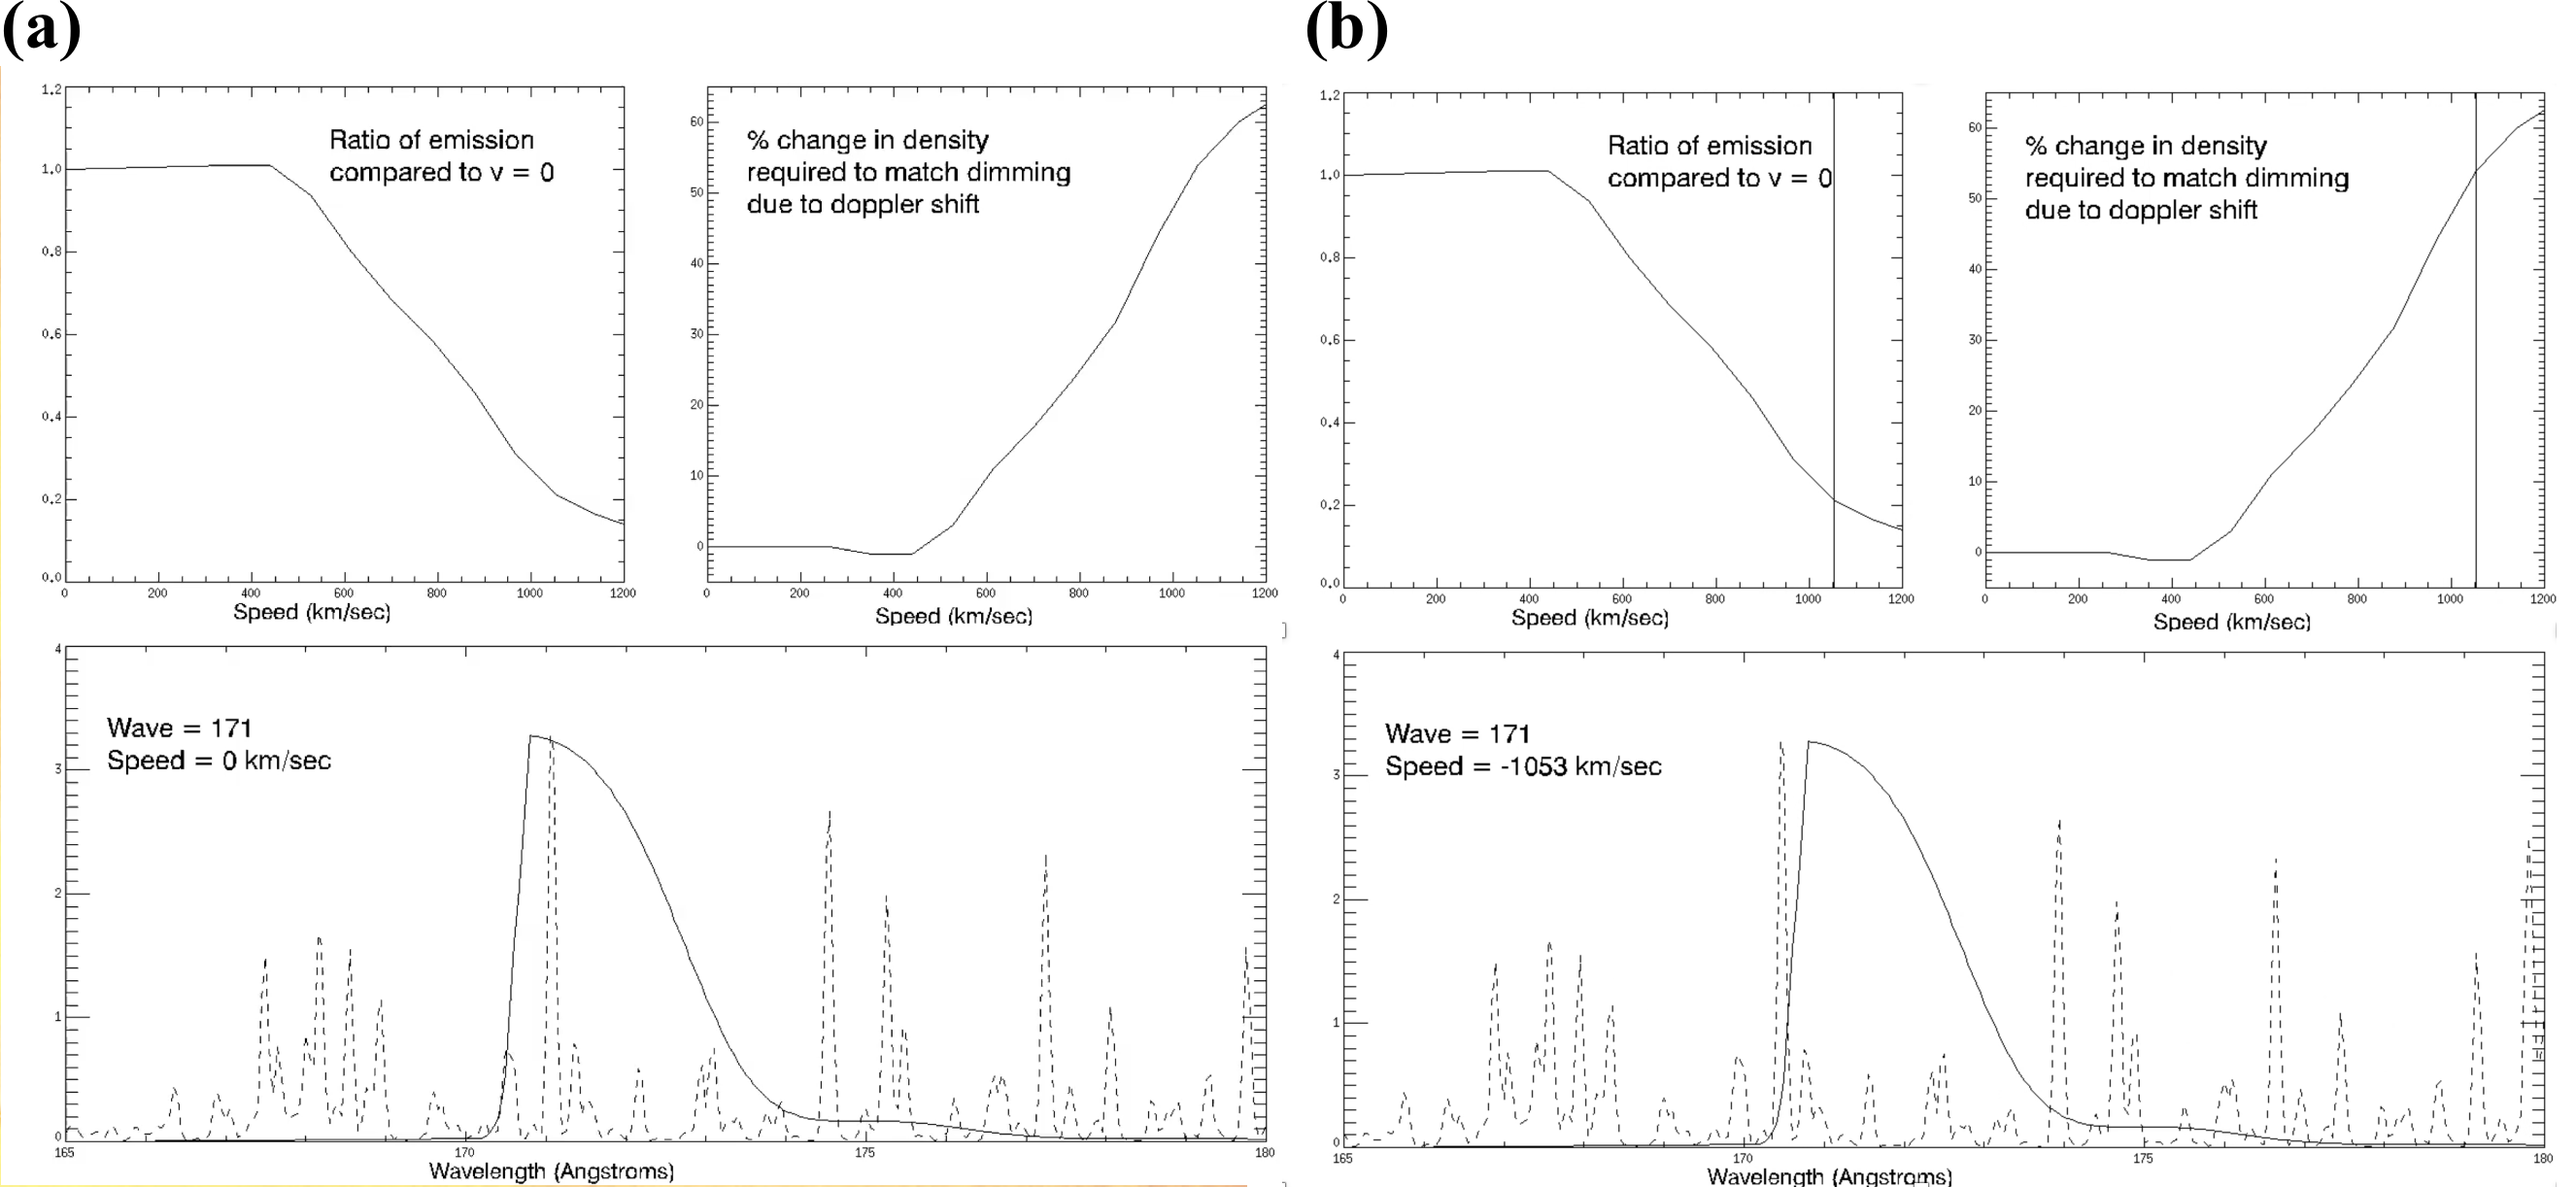
\includegraphics[width=166mm]{Images/BandpassDimming.png}
    \end{center}
    \label{bandpassDimming}
\end{figure}

\section{Summary}
Physics vs instrument effects

The physics for most of these types of dimming is relatively simple and well-understood, with the exception of global waves. Mass-loss dimming is simply the direct result of a CME removing a significant quantity of emitting material from the solar corona. This dimming is not immediately lost as the CME pulls away because the post-eruption relaxation period is nonzero and it can take several hours for the quiescent Sun to replace the lost plasma from the surrounding corona and transition region. Instrumentally, even though EUV measurements select specific temperature ranges, mass-estimates based on them appear consistent with white-light coronagraph derived masses \citep{Aschwanden2009}. 

Thermal dimming is a major concern in nearly all of the citations above for its potential to interfere with mass-loss dimming and the resultant estimated CME masses. The physics here is also simple: eruptive events result in various forms of heating (see Section \ref{sec:seePhysics}) that shift upward the ionization fraction of dominant EUV emitters (e.g., Fe). Instrumentally, this effect can be compensated for by measuring emission lines from multiple ionization states of the same ion (e.g., Fe IX-XV).

Obscuration dimming physics are also simple, essentially a result of Beer's law, as light passes through a medium with nonzero opacity. Instrumentally, this is easily identified with imagers and we believe it may be possible to identify with a spectrograph, provided some chromospheric helium emission lines are measured (e.g., 256 and/or 304 Å). 

The physics of global waves is highly contested but the observations are well established. For a disk-integrating spectrograph like EVE, which is the primary source of data analysis herein, we believe that wave dimming will be negated by wave brightening. Indeed, to our knowledge, no observations of waves have been made with EVE. 

Doppler dimming physics are well understood and long standing. A CME may fluoresce due to stimulation from the Sun, but the wavelengths will be Doppler shifted according to the relative velocity of the CME from the Sun. This shift reduces the efficacy of the stimulation, resulting in less fluorescence. However, the dimming region in this case is the CME itself, which is likely to be outside the field of view of instruments like AIA and EVE. Additionally, the emission lines of interest in this study are collisionally dominated. Thus Doppler dimming is an interesting phenomenon but is not expected to dramatically impact analyses of the other types of dimming. 

The physics of bandpass dimming is simple Doppler shifting of an emitting plasma. Potential dimming in this case is primarily an instrumental effect, as the Doppler shift could push important emission lines outside the instruments bandpass or data processing line-selection masks. However, studies have shown that the actual Doppler shifts are orders of magnitude too small to cause this type of dimming. 
